% Template for ISBI paper; to be used with:
%          spconf.sty  - ICASSP/ICIP LaTeX style file, and
%          IEEEbib.bst - IEEE bibliography style file.
% --------------------------------------------------------------------------
\documentclass{article}
\usepackage{spconf,amsmath,graphicx}

% It's fine to compress itemized lists if you used them in the
% manuscript
\usepackage{enumitem}
\setlist{nosep, leftmargin=14pt}

\usepackage{mwe} % to get dummy images
\usepackage{url}
% Example definitions.
% --------------------
\def\x{{\mathbf x}}
\def\L{{\cal L}}

% Title.
% ------
\title{Inference vs Retrieval- Evaluating Traditional Models and Novel Vector Classification Heuristics for Multimodal Garbage Classification}
%
% Single address.
% ---------------
\name{Maheen Hoque,$^{1}$ Arman Hossain Dipu Khan,$^{1}$ Lila Sanjay Kumar Gorlie$^{1}$}
\address{$^{1}$Master of Engineering Graduate Program, Electrical and Software Engineering, \\
 University of Calgary, Calgary, AB, Canada}
%
% For example:
% ------------
%\address{School\\
%	Department\\
%	Address}
%
% Two addresses (uncomment and modify for two-address case).
% ----------------------------------------------------------
%\twoauthors
%  {A. Author-one, B. Author-two\sthanks{Some author footnote.}}
%	{School A-B\\
%	Department A-B\\
%	Address A-B}
%  {C. Author-three, D. Author-four\sthanks{The fourth author performed the work
%	while at ...}}
%	{School C-D\\
%	Department C-D\\
%	Address C-D}
%
% More than two addresses
% -----------------------
%\name{Author Name$^{\star \dagger}$ \qquad Author Name$^{\star}$ \qquad Author Name$^{\dagger}$}

%\address{$^{\star}$ Affiliation Number One \\ $^{\dagger}$}Affiliation Number Two
%
%\name{Author Name$^{\star \dagger}$ \qquad Author Name$^{\star}$ \qquad Author Name$^{\dagger}$}

%\address{$^{\star}$ Affiliation Number One \\ $^{\dagger}$Affiliation Number Two}
\begin{document}
%\ninept

\maketitle
%
\begin{abstract}

With the increasing use of multimodal data and specialized models for classification tasks, important questions arise regarding the effectiveness of traditional inference-based models versus retrieval-augmented approaches. In particular, combining image and text modalities introduces challenges in achieving both accuracy and robustness, especially when it comes to data skewness and domain drift (and additional training resource cost when comparing with ). In this work, we compare supervised multimodal models with retrieval-augmented classification using 3 novel vector-based heuristics for four-class garbage classification problem. Through our various experiments, we found that, while supervised fusion models provide strong baseline performance and inference velocity, retrieval-based methods, especially density-aware approaches, show improved robustness and better performance (upto 3.41\% in F1 Score, without any additional tuning) under severe class imbalance and limited memory conditions.

\end{abstract}
%
\begin{keywords}
Multimodal Lerning, Garbage Classification, RAC (Retrieval-Augmented Classification), Vector Heuristics, DNDS (Density Normalized Distance Score), Deep Learning.
\end{keywords}
%

\section{Introduction}
\label{sec:intro}

Garbage classification is an intriguing field that offers a good opportunity for applied multimodal classification tasks, as waste management facilities regularly use machine learning \cite{alexakis2025enhanced} to sort garbage according to some predefined criteria. The sorting typically implements unimodal classification with garbage images. But additional modality of text can help with ambiguity of classification that may arise with a single modality of images. 

Deep learning (DL) models have been a popular choice in multimodal classification due to their ability to learn from heterogeneous data sources such as images and text and being more adaptable for complex patterns than traditional machine learning models. By leveraging complementary information across modalities, multimodal approaches often outperform unimodal systems. A common strategy is combine predictions from image and text models using fusion techniques such as weighted logic aggregation, enabling improved accuracy and generalization. However, these supervised approaches rely entirely on learned representations and may face limitations under challenging conditions such as class imbalance, limited training data or domain drift. Those conditions often require rigorous training, normalization, complex feature engineering, augmentation, or re-training an existing model - which means a penalty of computational resources on top of an already extensive dataset required for these models to work properly \cite{islam2026learning} \cite{alexakis2025enhanced}.

An alternative approach is retrieval-augmented classification (RAC), which utilizes embedding-based memory to retrieve similar instance and make predictions based on neighborhood evidence. This allows the model to incorporate additional contextual information beyond the training distribution but introduces challenges in retrieval design and scoring. Despite increasing interest in such methods, a systematic comparison between traditional supervised inference and retrieval-based approaches remains limited. In our work, a two-phase framework is presented to evaluate both strategies for multimodal garbage classification, with experiments conducted under standard settings, class imbalance, and varying memory size to analyze performance, robustness, and generalization. Implemented with modern vector databases like Chroma, Pinecone, LanceDB, and PGVector - RAC only has a storage overhead, which is much cheaper than memory in terms of hardware price. 

But more importantly, to address the challenges in retrieval design and scoring, we propose a novel heuristic - Density Normalized Distance Score (DNDS) that specifically addresses the challenge of data skewness or imbalance, and domain drift by taking into account class distributions in various ways. This DNDS has 3 variants that we studied in this work - Global DNDS (takes the entire database into account for class imbalance), Local DNDS (takes into account a local region of a query for class imbalance), and KDE DNDS (Uses Gaussian kernel density estimation for accounting ``instance contribution" for class imbalance). This DNDS heuristic is dynamic (works well even with continuously increasing database size), designed to work with cosine distances with high-dimensional vector embedding, and corrects itself for class skewness. Throughout this study, we focused more over evaluating these 3 variants of the DNDS heuristic, with a traditional deep learning approach involving a 2 step approach implemented with MobileNetV3 and DistilBERT. Now, our research questions (RQ), that we tried to answer in this study is as follows:     

\begin{itemize}
  \item \textbf{RQ 1}: Does DNDS have better performance compared to traditional methods for classification? 
  \item \textbf{RQ 2}: How robust is DNDS against severe class imbalance?
  \item \textbf{RQ 3}: Can DNDS maintain it's performance with increasing database size?
  \item \textbf{RQ 4}: Which DNDS variant is the most effective overall?
\end{itemize}

\begin{figure}[htb]
\centering
\centerline{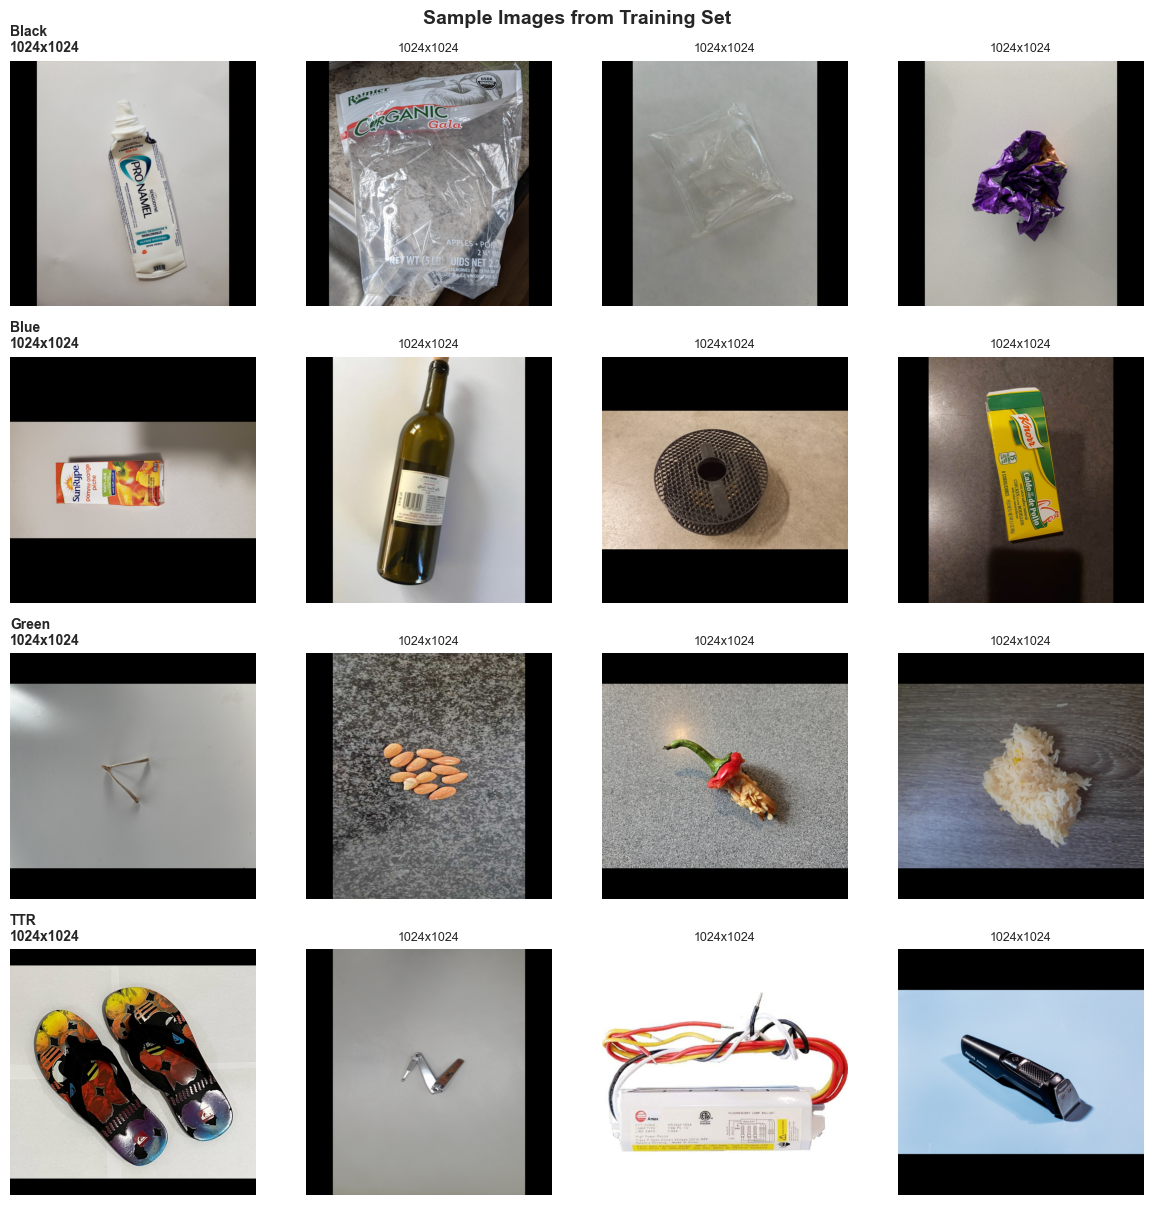
\includegraphics[width=\linewidth]{images/Classification.png}}
\caption{Sample images from the training dataset across four classes- Black, Blue, Green, and TTR-demonstrating the diversity of objects and visual variations within each category.}
\label{fig:classification}
\end{figure}

\section{Methods}
\subsection{Datasets}
The CVPR 2024 trash classification dataset was used for training, validation, and testing of both supervised and retrieval-based models. The task involves four-class classification of garbage categories: Black, Blue, Green, and TTR as shown in Figure \ref{fig:classification}. The dataset contains images and text data, where text inputs are derived from filename-based descriptions and serve as an additional modality.

The image dataset is organized into training, validation, and test splits, ensuring proper separation for model development and evaluation. Corresponding text data are provided in CSV format with labeled samples aligned to the image data. All images were resized and normalized before training, while text data were tokenized and processed using standard natual language preprocessing techniques.

To improve generalization, the dataset was used in multiple experimental settings. In addition to standard training, and testing, class imbalance scenarios were simulated by reducing the number of samples in minority classes at controlled ratios. Futhermore, for retrieval-based experiments, multimodal embeddings from the training and validation sets were stored in a persistent database, which was progressively expanded to study the impact of memory size on performance.

\subsection{Model Architectures}
Two categories of approaches were evaluated: supervised multimodal models and retrieval-augmented classification (RAC)

For supervised learning, an image model based on MobileNetV3 and a text model based on DistilBERT were trained independently. Their outputs were combined using weighted logic fusion to leverage complementary information from both modalities. The fusion is defined as:
  \begin{center}
      $W_{fused} = \alpha W_{text}+(1-\alpha)W_{image}$
  \end{center}    
were $W_{text}$ and $W_{image}$ are the class scores from text and image models, respectively, and $\alpha \in [0,1]$ controls the contribution of each modality.

In addition to supervised models, retrieval-augmented classification was implemented using multimodal embedding stored in a ChromaDB database. For a given query $q$, nearest neighbors are retrieved separately for image and text modalities, and class scores are computed using different vector-based heuristics.

The final RAC prediction is obtained by combining modality-specific scores:
  \begin{center}
      $S(c) = \alpha S_{I}(c)+(1-\alpha)S_{T}(c)$,\quad $\hat{y} = \arg\max_{c} S(c)$
  \end{center} 
where $S_{I}(c)$ and $S_{T}(c)$ denote image and text retrieval scores.
Several scoring strategies were evaluated:
Majority vote:
  \begin{center}
      $S_{m}(c) = S_m(c) = \sum_{i \in N_k^{(m)}(q)} \mathbf{1}[y_i = c]$
  \end{center} 
Inverse Distance Weighting (IDW):
  \begin{center}
      $S_{m}(c) = S_m(c) = \sum_{i \in N_k^{(m)}(q),y_{i}=c} \frac{1}{d_k^{m} + \epsilon} $
  \end{center} 
Global Density Normalized Distance Scaling (Global DNDS):
  \begin{center}
      $\rho_m(c) = \frac{N_m(c)}{\sum_{c'} N_m(c')},$ \\ \vspace{10pt}
$S_m(c) = \sum_{\substack{i \in \mathcal{N}_k^{(m)}(q) \\ y_i = c}} 
\frac{1}{\left(d_i^{(m)} + \epsilon\right)\,\rho_m(c)}$
  \end{center} 
Local Density Normalization (Local DNDS):
  \begin{center}
      $\rho_m^{\text{local}}(c) = 
\frac{\left| \{ i \in \mathcal{N}_{K_{\text{density}}}^{(m)}(q) : y_i = c \} \right|}
{K_{\text{density}}}$,\\ \vspace{10pt}
$S_m(c) = 
\frac{
\sum_{\substack{i \in \mathcal{N}_k^{(m)}(q) \\ y_i = c}} 
\frac{1}{d_i^{(m)} + \epsilon}
}
{\rho_m^{\text{local}}(c)}$
  \end{center}
KDE-Based Density Normalization (KDE-DNDS):
  \begin{center}
      $\tilde{\rho}_m(c) = \sum_{j : y_j = c} 
\exp\left( -\frac{\left(d_j^{(m)}\right)^2}{2h^2} \right)$, \\ \vspace{10pt}
$S_m(c) =\frac{\sum_{\substack{i \in \mathcal{N}_k^{(m)}(q),,  y_i = c \frac{1}{d_i^{(m)} + \epsilon}}}} 
{{\tilde{\rho}_m(c)}}$
  \end{center} 
where $d_i^{(m)}$ represents the distance of neighbor i,$\epsilon$ is a small constant for numerical stability, and $h$ is the KDE bandwidth.

These formulations allow comparison between traditional inference-based models and retrieval-based decision rules, highlighting the impact of density-aware normalization on classification performance and robustness.

\subsection{Experimental setup and procedure}
All models were trained and evaluated under consistent settings. Hyperparameters such as fusion weight $(\alpha)$, neighborhood size $(k)$, and density parameters were tuned using validation set. Performance was measured using accuracy, macro F1-score, weighted F1-score, and per-class percision and recall.  

To evaluate robustness, controlled imbalance experiments were conducted by reducing class samples at predefined ratios. Additionally, a continual-memory setup was implemented where the retrieval database size was gradually increased to analyze performance trends. These experiments provide insights into the eddectiveness of supervised and retrieval-based approaches in terms of accuracy, robustness, and generalization.

\begin{figure}[htb]
\centering
\centerline{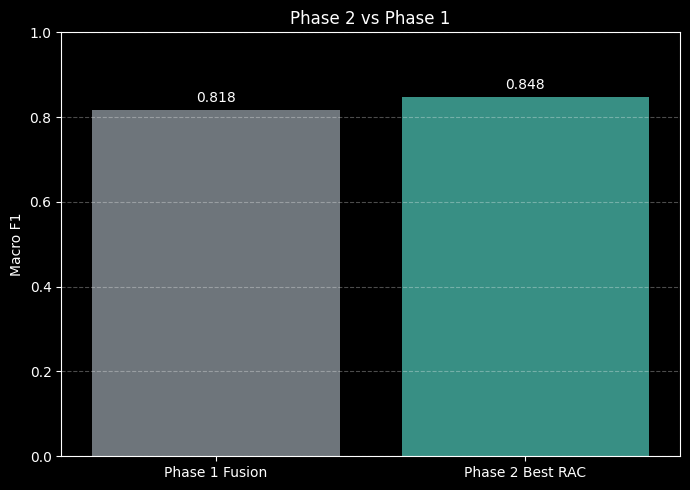
\includegraphics[width=\linewidth]{images/phase 1 vs 2.png}}
\caption{Comparison of Phase 1(supervised fusion) and Phase 2(retieval-augmented classification), showing improvement in macro F1 score.}
\label{fig:phase}
\end{figure}

\begin{figure}
\centering
\centerline{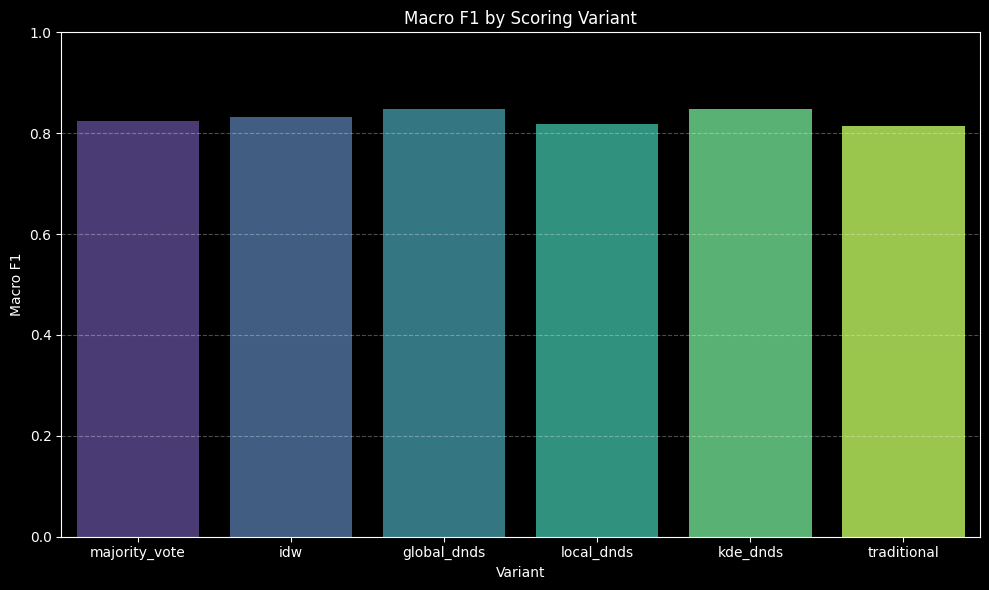
\includegraphics[width=\linewidth]{images/Macro F1 scoreing variant.png}}
\caption{Macro F1 score cmparison across different scroing variants, highlighting the effectiveness of density-aware methods.}
\label{fig:macro_variant}
\end{figure}

\begin{figure}
\centering
\centerline{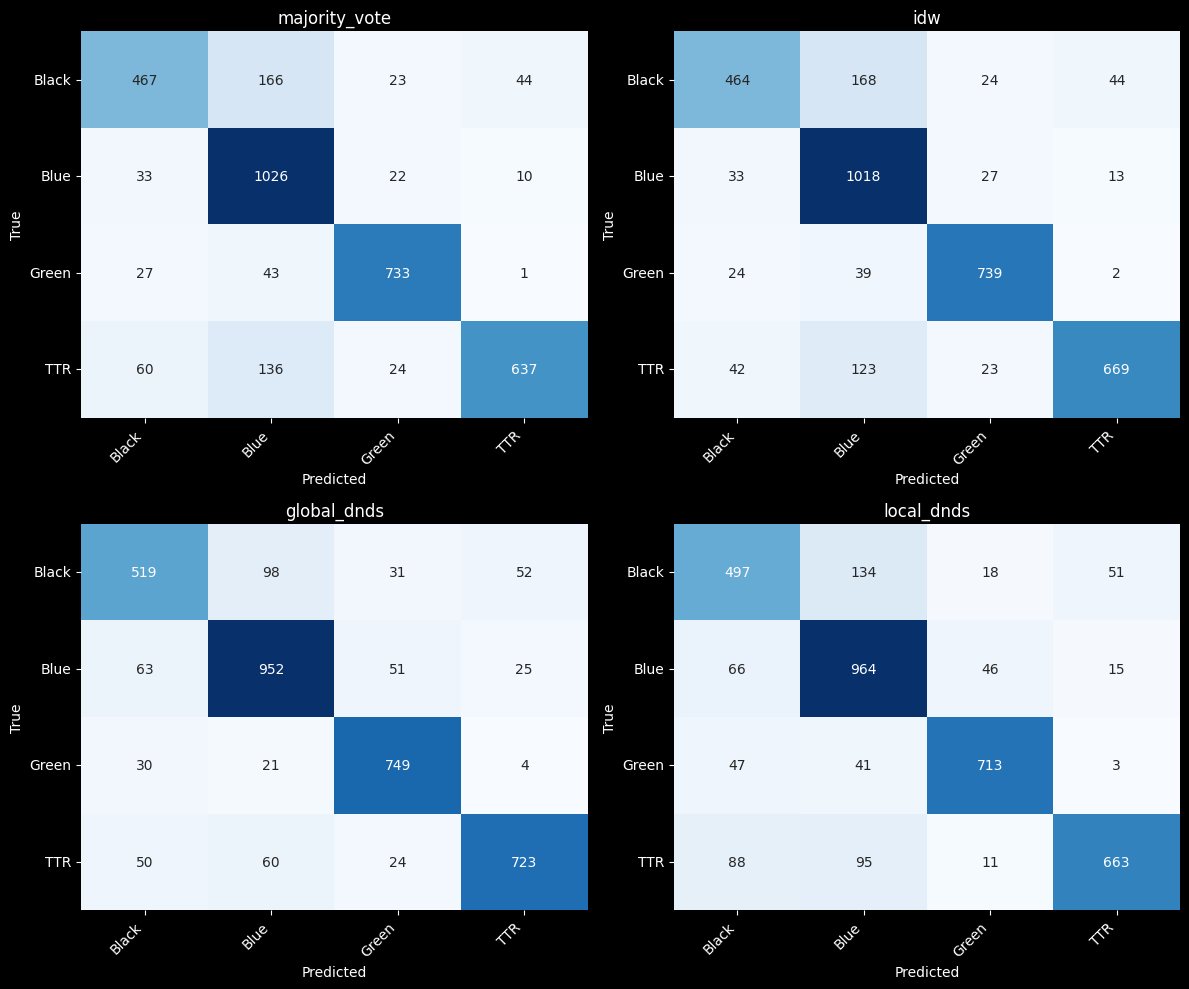
\includegraphics[width=\linewidth]{images/confusion matrix.png}}
\caption{Confusion matrices for different scoring methods, illustrating classification performance across all classes.}
\label{fig:confusion}
\end{figure}

\begin{figure}
\centering
\centerline{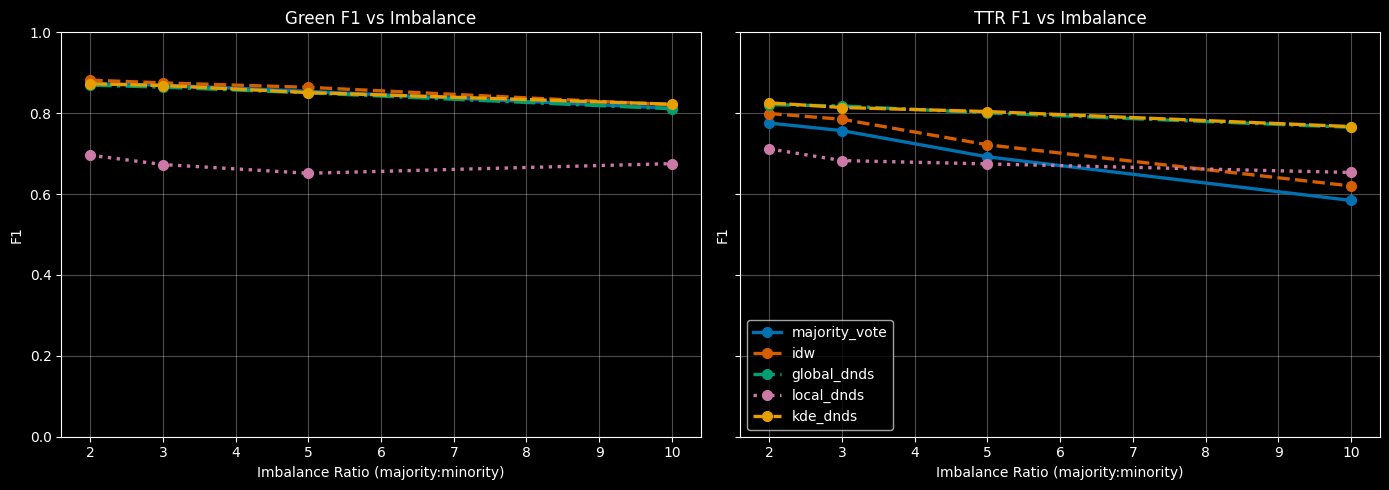
\includegraphics[width=\linewidth]{images/imbalance.png}}
\caption{Class-wise F1 score under increasing imbalance ratios, demonstrating improved robustness of density-aware methods.}
\label{fig:imbalance}
\end{figure}

\begin{figure}
\centering
\centerline{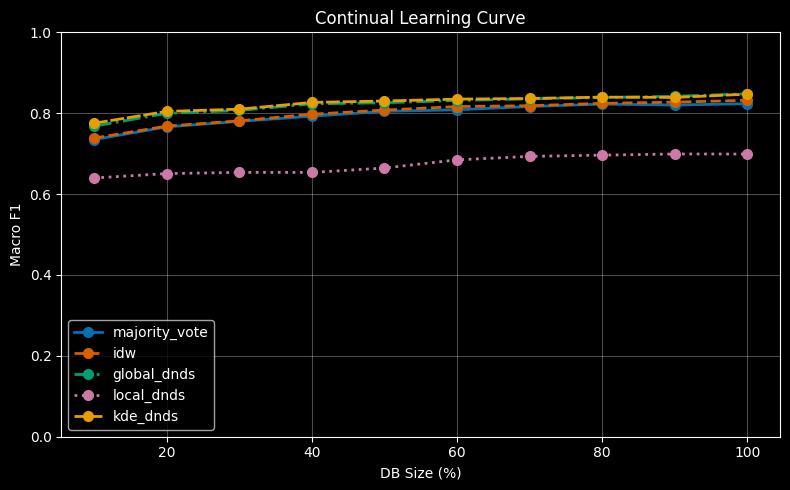
\includegraphics[width=\linewidth]{images/learning curve.png}}
\caption{Macro F1 score as a function of retrieval database size, showing performance improvement with increasing memory.}
\label{fig:learning}
\end{figure}

\section{Results}
Figure \ref{fig:phase} showing improvement in macro F1 score. Phase 2 demonstrates clear improvement over Phase 1, including the effectiveness of retrieval-based methods.Figure \ref{fig:macro_variant} Macro F1 score comparison across different variants, highlighting the effectiveness of density-aware methods. Density-based methods(global DNDS, KDE-DNDS) achieve the hightest performance, outperforming majority voting and IDW.Figure \ref{fig:confusion} demonstrates different scoring methods, illustrating classification performance across all classes. Density-aware methods show better class-wise accuracy, particularly for challenging classes like TTR. Figure \ref{fig:imbalance} demonstrating improved robustness of density-aware methods. Performance degrades with imbalance, but density-based methods remain more stable. Figure \ref{fig:learning} Macro F1 score as a function of retrieval database size, showing performance improvement with increasing memory. All methods improve with large memory, with density-aware approaches showing more consistent gains.

\section{Discussion}
Across standard evaluation settings, retrieval-augmented classification demonstrates a clear and consistent improvement over traditional supervised fusion models. While multimodal fusion effectively combines image and text information to produce string baseline results, it relies entirely on learned representations and may not fully capture complex relationships in the data. In contrast, retrieval-based approaches leverage embedding neighborhood, allowing predictions to be influenced by similar examples. Among the evaluated methods, density-aware heuristics such as global DNDS and KDE-DNDS achieve the highest performance, indicating that incorporate class density into scoring leads to more reliable and discriminative predictions. Simpler approaches such as majority voting and inverse distance weighting show comparatively lower performance, highlighting their limitations in handling overlapping class distributions.

Under class imbalance conditions, all methods experience a decline in performance; however, the extent of degradation varies significantly. Density-normalized approaches maintain substantially higher F1 scores for minority classes, particularly TTR, demonstrating improved robustness. This behavior suggests that density-aware methods effectively compensate for uneven class distributions by reducing the dominance of majority-class neighbors during retrieval. In contrast, non-normalized methods tend to bias predictions towards majority classes, leading to increased misclassifications. The confusion matrix analysis further supports these findings, showing that density-based methods achieve better class separation and reduced confusion between visually or semantically similar categories.

In the continual-memory experiments, performance improves as the size of the retrieval database increases, confirming the importance of richer neighborhood information. As more samples are added, the embedding space becomes more representative of the overall data distribution, enabling more accurate retrieval and classification. Density-based methods exhibit more stable and consistent improvements compared to other approaches,indicating their ability to effectively utilize additional data without being adversely affected by redundancy or imbalance. This highlights a key advantage or retrieval-based system: their performance can scale with data availability without requiring retaining.

The observed performance differences can be attributed to how each method handles local and global data structure. Density-aware heuristics explicitly normalize scores based on class distribution, reducing bias and improving generalization. In contrast, simpler heuristics rely solely on distance or count-based measures, which may not adequately reflected the true distribution of classes in the embedding space. Additionally, retrieval-based methods introduce flexibility by allowing the system to adapt dynamically to new data through memory expansion, unlike traditional models that require retraining for updates.

Overall, while supervised multimodal fusion provides a strong and efficient baseline, retrieval-augmented classification particularly with density normalization offers improved robustness, scalability, and generalization. These findings suggest that combining inference-based learning with retrieval-driven reasoning is a promising direction for multimodal classification tasks. Future work may explore more advanced embedding techniques, adapting retrieval strategies, and hybrid models that further integrate supervised learning with retrieval mechanisms to enhance performance accross diverse real-word scenarios.

\section{Conclusion}
\label{sec:majhead}
In this work, we investigated the effectiveness of supervised multimodal fusion and retrieval-augmented classification for garbage classification. We found that while supervised fusion models provide strong baseline performance, retrieval-based approaches, particularly density-aware methods, achieve improved accuracy and robustness. These methods demonstrate better performance under class imbalance and benefit from increased retrieval memory, indicating their scalability and adaptability.

Overall, the results suggest the retrieval-augmented classification offers a more reliable and generalizable approach compared to traditional inference-based models. This highlights the importance of integrating retrieval mechanisms with multimodal learning for real-world classification tasks. \cite{zhang2013support} \cite{pedregosa2011scikit}

% To start a new column (but not a new page) and help balance the last-page
% column length use \vfill\pagebreak.
% -------------------------------------------------------------------------
%\vfill
%\pagebreak

\clearpage

\section{Acknowledgments}
\label{sec:acknowledgments}
ND is supported by an Natural Sciences and Engineering Research Council (NSERC) BRAIN CREATE award, an NSERC Canada Graduate Scholarship (CGS-M), an Alberta Innovates graduate student award, and an Alberta Graduate Excellence Scholarship (AGES). RS and RF thank NSERC for ongoing operating support for this project (RGPIN/2021-02858 and RGPIN/2021-02867). RS also acknowledges operational support from the NSERC Alliance–Alberta Innovates Advance Program.

% References should be produced using the bibtex program from suitable
% BiBTeX files (here: strings, refs, manuals). The IEEEbib.bst bibliography
% style file from IEEE produces unsorted bibliography list.
% ------------------------------------------------------------------------- 

\bibliographystyle{IEEEbib}
\bibliography{strings,refs}

\end{document}
